\documentclass{article}

\usepackage{listings}
\usepackage{color}
\usepackage{graphicx}
\usepackage{float}
\usepackage{amsmath}
\usepackage{subfig}
\usepackage{cite}
\usepackage{url}
\usepackage{amsmath}

\begin{document}

\title{Image Analysis - TP3 - Feature detection}

\author{Jander Nascimento, 
\and Raquel Oliveira}

\maketitle

\section{Gradient Images}
	
	\subsection{Horizontal and vertical gradient}

	The gradient is created based on a vector that points to the highest rate of change in the magnitude, and can be represented as in the Formula \ref{eq:gradient}. 

\begin{equation}
\bigtriangledown f = \begin{pmatrix}
\frac{\partial f}{\partial x} = G_x\\ 
\frac{\partial f}{\partial y} = G_y
\end{pmatrix}
\label{eq:gradient}
\end{equation}

The gradient can be reached in several manners, the performance and accuracy constraints may dictate which method best fits. 

For this specific project, the method adopted was a kernel convolution with the sobel operator, that is an approximation of the integral. 

The both sobel operators, horizontal and vertical, can be seen in the the Table \ref{tab:sobelx} and \ref{tab:sobely}. Each of them are applied individually to the source image to produce different images.

\begin{figure}
  \begin{center}
  \subfloat[Horizontal]{
  \begin{tabular}{ | c | c | c | }
    \hline
    -1 & -2 & -1 \\ \hline
    0 & 0 & 0 \\ \hline
    1 & 2 & 1 \\
    \hline
  \end{tabular}\label{tab:sobely}}
  \subfloat[Vertical]{
  \begin{tabular}{ | c | c | c | }
    \hline
    -1 & 0 & 1 \\ \hline
    -2 & 0 & 2 \\ \hline
    -1 & 0 & 1 \\
    \hline
  \end{tabular}\label{tab:sobelx}}
  \end{center}
  \caption{$G_y$ and $G_x$ sobel operator}
\end{figure}

There exist several filters that can be used to find the gradient. e.g: sobel and prewitt. Here was used the sobel operator to reach the results.

The sobel operator is a pair of kernels (one for vertical and one horizontal detection) which can be convolved with the source image to obtain its gradient.

In the Figure \ref{fig:gradient} we can see the result of the horizontal and vertical gradients.

	\begin{figure}[H]
	\centering
	\subfloat[Original Image]{\label{fig:original}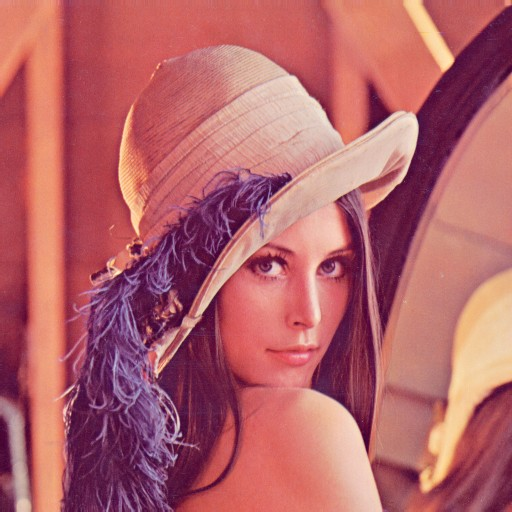
\includegraphics[width=0.3\textwidth]{../lena}}                
	\subfloat[Horizontal Gradient]{\label{fig:horizontal}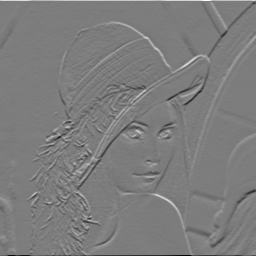
\includegraphics[width=0.3\textwidth]{../img/lena_gradienty}}                
	\subfloat[Vertical Gradient]{\label{fig:vertical}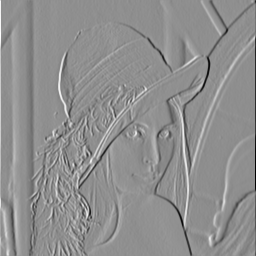
\includegraphics[width=0.3\textwidth]{../img/lena_gradientx}}                
	\caption{Gradient}
	\label{fig:gradient}
	\end{figure}


\section{Gradient Norm}

Gradient Norm is the representation of the gradient normal vector. This can be reached through one of the two Equations \ref{equa:norm1} or \ref{equa:norm2}.

The result of the Gradient Norm can be seen in the Figure \ref{fig:norm_gradient}. 

\begin{figure}[H]
	\centering
	\subfloat[Horizontal Gradient]{\label{fig:norm_horizontal}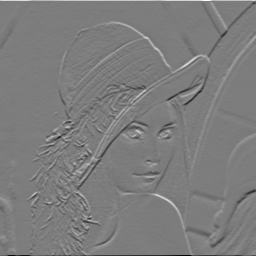
\includegraphics[width=0.3\textwidth]{../img/lena_gradienty}}                
	\subfloat[Vertical Gradient]{\label{fig:norm_vertical}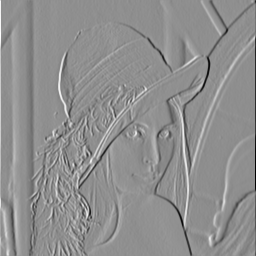
\includegraphics[width=0.3\textwidth]{../img/lena_gradientx}}                
	\subfloat[Gradient norm]{\label{fig:norm}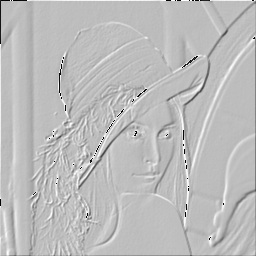
\includegraphics[width=0.3\textwidth]{../img/lena_gradientxy}}                
	\caption{Gradient}
	\label{fig:norm_gradient}
\end{figure}

%\begin{equation}
%magn(\bigtriangledown f) = \sqrt{M_x^{2}+M_y^{2}}\approx \left | M_x \right |+\left | M_y \right |
%\label{equa:norm}
%\end{equation}

\begin{equation}
G = \sqrt{G_x^{2}+G_y^{2}}
\label{equa:norm1}
\end{equation}

\begin{equation}
G = | G_x | + | G_y |
\label{equa:norm2}
\end{equation}

Both Equations are valid, but once more the computational costs differs from one to another.

\section{Corner Detection}
	
	Feature detection is an approach in Image Analysis that can extract interest points from the image. An interest point is a point in an image which has a well-defined position and can be robustly detected. Interest points can be corners, T-junctions or points with high texture variations. A large amount of interest points detectors has been already proposed in the literature. In practice, most so-called corner detection methods detect interest points in general, rather than corners in particular. However, most of these works assume that key points are equivalent to points characterized by a significant gradient amount in more than one direction.

	The one of the earliest corner detector was Moravec. This operator computes the average change in image intensity, \textit{E(x,y)} when a window \textit{W} is shifted around a pixel \textit{(x,y)} in several directions. In an homogeneous region, \textit{E} is small for any displacement. When located on an edge pixel, the minimum value of \textit{E} is related to the edge direction and so is also small. But for corner pixel or a more complicated junction, any displacement results in a non zero value for \textit{E}.
	
	\textit{E} is thus defined as follows:

	\begin{equation}
	E_(x,y) = \sum_{u,v} w_{u,v} |I_{x+u,y+v} - I_{u,v}|^2
	\end{equation}

	where \textit{I} is the input image and \textit{w} is the local window.
	\\\\
	The main problem with Moravec detector is that it considers only a small set of possible shifts, which means that if an edge is present that is not in the direction of the neighbors, then it will not be detected as an interest point. This problem was solved in the Harris corner detector (Harris and Stephens, 1988) by extending this measure to any directions using a Taylor expansion about the shift origin, i.e. for small shifts (x,y):

	\begin{equation}
	E(x,y) = \sum_{u,v} w_{u,v}   |x \frac{\partial I}{\partial x} + y \frac{\partial I}{\partial y} + O(x^2,y^2)|^2
	\end{equation}

	\begin{equation}
	E(x,y) = Ax^2 + 2Cxy + By^2
	\end{equation}
	
	where:
	
	\begin{equation}
	A = \frac{\partial I}{\partial x} * w
	\end{equation}

	\begin{equation}
	B = \frac{\partial I}{\partial y} * w
	\end{equation}

	\begin{equation}
	C = \frac{\partial I}{\partial x} \frac{\partial I}{\partial y} * w
	\end{equation}

	and  * means the convolution product.
	\\\\
	If a circular window (or circularly weighted window, such as a Gaussian) is used, then the response will be isotropic, which means that even if an edge is present that is not in the direction of the neighbors, it will be detected as an interest point.

	The Equation can be rewritten as:

	\begin{equation}
	E(x,y) = (x,y)M(x,y)^t
	\end{equation}
	
	with:

	\begin{equation}
	M = 	\begin{bmatrix}
		A&C\\
		C&B
		\end{bmatrix}
	\end{equation}

	Based on the behavior of the eigen values of \textit{M}, Harris and Stephens proposed the following formula:

	\begin{equation}
	H = det(M) - \alpha trace(M)^2
	\end{equation}

	with: \textit{det(M) = AB-$C^2$} and \textit{trace(M) = A+B}
	\\\\
	The number of detected corners (local positive maxima of H) highly depends on the value of the parameter \textit{$\alpha$}. As greater \textit{$\alpha$} is, as greater the number of corner are detected.
	
	In Figure \ref{fig:harris} we can see one example of the Harris Detector applied in an image.

	\begin{figure}[H]
	\centering
	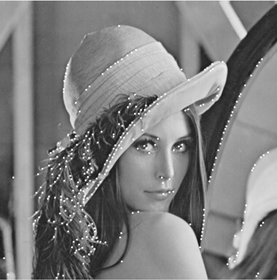
\includegraphics[width=0.3\textwidth]{../img/lennaharris}
	\caption{Harris Operator}
	\label{fig:harris}
	\end{figure}
	
	\subsection{How to run?}

	Steps to compile the application:
	
	\begin{itemize}
		\item svn checkout https://jfimageanalysis.googlecode.com/svn/trunk/TP2/ \#download source code
		\item make \#compiles the code
	\end{itemize}

	{\bf Pgm plaintext} files are the only file type accepted (P2). 

	Examples of usage:

	\begin{itemize}
		\item Harris corner detection:
		\subitem ./imagetransform -f harris -i image\_in.pgm $>$ image\_out.pgm
	\end{itemize}

	You can always type {\it ./imagetransform --help} to check for more options. 


\end{document}


